\section{\label{results}Results}

\subsection{\label{faster_is_slower}The faster is slower effect}


As a starting point, we checked over the ``faster is slower'' effect for 
the room with two doors on the same wall. Fig.~\ref{fig:7} shows the 
recorded evacuation time when the doors are separated a distance of $d_g=1\,$m 
and when no separation exists at all ($d_g=0$). The latter means a single 
opening with width equal to two doors. Both cases (with or without separation) 
exhibit a change in their corresponding slopes. Thus, the ``faster is 
slower'' effect is achieved following the same qualitative response as the one 
found in previous works for rooms with a single exit \cite{Helbing1,Dorso1}.\\ 


\begin{figure}
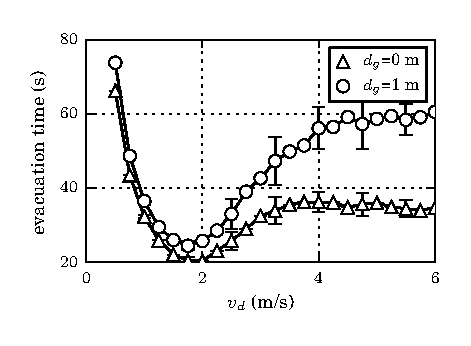
\includegraphics[width=\columnwidth]{./fig1.eps}
\caption{\label{fig:7} Mean evacuation time for 160 individuals (seconds) 
vs. the pedestrian's desired velocity (m/s). The room was $20\times20\,$m 
size. Two contiguous doors were placed on one side of the room as shown in 
Fig.~\ref{fig:19} (see text for details). Mean values were computed from 30 
evacuation processes. Each door was $d_w=1.2$~m width. The desired velocity 
was $v_d=4\,$m/s. Two situations are shown:  $\bigtriangleup$ corresponds to 
the null separation distance between doors, meaning a single door of $2d_w$ 
width. $\bigcirc$ corresponds to the 1~m separation distance between doors  
($d_g=1$~m).   }
% done with fig7_version0.py 
\end{figure}


The evacuation time for separated doors in Fig.~\ref{fig:7} is always above the 
time required to evacuate the pedestrians through the single opening 
(\emph{i.e.} null separation). For $v_d=6\,$m/s, the single opening improves 
the evacuation performance in half of the time that demands the $d_g=1\,$m 
separation configuration. Other separation distances (not shown) exhibit the 
same qualitative pattern as the example presented in Fig.~\ref{fig:7}. 
Therefore, it is clear that while the total width of the opening 
remains unchanged, splitting this width into to symmetric exits affects 
significantly the evacuation performance. \\

We made further research on the $d_g=0$ and $d_g>0$ scenarios. The 
former is investigated in Section \ref{single_double}, while the latter is left 
to Section \ref{door_seperation}. \\

\subsection{\label{single_double}The single door vs. the null separation}

Recall that the $d_g=0$ scenario corresponds to a single opening, but the total 
width of the opening is twice the width of a single door (see 
Section~\ref{faster_is_slower}). Actually, it resembles the situation of a 
double sheet door.  \\

\subsubsection{\label{null_gap_data}The stop-and-go process}

Fig.~\ref{fig:8and9} illustrates on how the evacuation performance improves as 
the opening becomes wider.  Fig.~\ref{fig:9} corresponds to the single door 
($d_w=1.2\,$m), while  Fig.~\ref{fig:8} corresponds to a wider opening 
($3d_w=3.6\,$m), resembling a multi-leaf opening. Both figures represent 
the time evolution of a single pedestrian during an evacuation process. We can 
see the (normalized) pressure acting on the pedestrian and his (her) 
corresponding velocity. The starting point of the pedestrian was 
$(x,y)=(12.35\,\mathrm{m},8.45\,\mathrm{m})$. Notice that an increase in the 
opening width from $d_w$ to $3d_w$ (Fig.~\ref{fig:9} and Fig.~\ref{fig:8}, 
respectively) reduces the evacuation time by one-fifth approximately. \\

\begin{figure*}[!htbp]
\subfloat[Opening of $d_w=1.2$~m width.\label{fig:9}]{
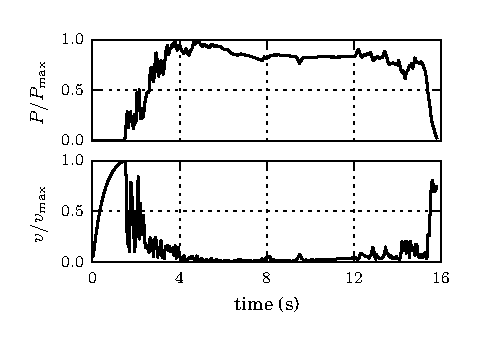
\includegraphics[width=0.75\columnwidth]{./fig2.eps}
% done with fig9_version0.py 
}\hfill
\subfloat[Opening of $3d_w=3.6$~m width. \label{fig:8}]{
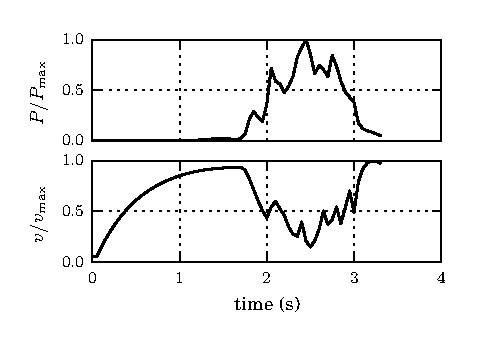
\includegraphics[width=0.75\columnwidth]{./fig3.eps}
% done with fig8_version0.py 
}
\caption{\label{fig:8and9} Normalized pressure and velocity on a single 
pedestrian during an evacuation process. Data was recorded from the 
the initial position at $x=12.35$~m and $y=8.45$~m, until the individual left 
the room ($x>20$~m).  The pedestrians desired velocity was $v_d=4\,$m/s. Two 
situations are shown: (a) evacuation through a single door of width 
$d_w=1.2$~m. (b) evacuation through an opening of $3d_w=3.6$~m.} 
\end{figure*}


The pedestrian represented in Fig.~\ref{fig:8and9} increases his (her) 
velocity towards an asymptotic value at the beginning of the processes. This 
value corresponds to the desired velocity $v_d=4\,$m/s. But close to $t=2\,$s, 
the pedestrian suddenly stops because of the clogging around the exit. Clogging 
is also responsible for the pressure increase, as shown in both Fig.~\ref{fig:9} 
and Fig.~\ref{fig:8}. This can be checked over by means of Eq.~(\ref{eqn_2}) 
because when the velocity of the pedestrian vanishes, the desire force 
$\mathbf{f}_d$ attains a maximum (in panic situations only). Notice, however, 
that any further fluctuation of the pressure acting on the pedestrian 
corresponds to an inverse fluctuation on the velocity. Thus, the pedestrian is 
able to reach the exit following a stop-and-go 
process. \\

The instantaneous pressure acting on a single pedestrian can be computed from 
Eq.~(\ref{eqn_4b}) for a slow moving pedestrian (that is, $p_i\simeq 0$). 
The maximum pressure values $\mathrm{P}_\mathrm{max}$ in 
Fig.~\ref{fig:9} and Fig.~\ref{fig:8} are 8550~N.m$^{-1}$ and 6475 N.m$^{-1}$, respectively. 
The corresponding mean pressure values (after the first $2\,$s) are 80\% and 
55\% of the respective maximum values. This means that the mean pressure value for the 
$3d_w$ situation is lower than the corresponding mean value for the $d_w$ situation. 
% This statment is restricted to pedestrians that evacuate through the middle of the room.
That is, the wider opening seems to release pressure from time to time. Consequently, 
the stop-and-go processes are somehow different for the 
single door with respect to the $d_g=0$ situation (the wider opening). \\

\subsubsection{\label{null_gap_patterns}The pressure and stream patterns}

For a better understanding on how the pedestrians are (intermittently) released 
from high pressures in the wide opening situation, we pictured the whole scene 
into a pressure contour map and a mean stream path map for all the individuals. 
Fig.~\ref{fig:3} shows the pressure levels ($P_i$) for the 
clogging area. The warm colors are associated to high pressure values. These 
values are close to the corresponding maximum pressure values (not shown). Thus, 
the warm regions define the places where the pedestrians slow down most of the 
time. They are expected to get released only for short periods of time. On the 
contrary, the regions represented in cold colors (low mean pressure) are those 
where the individuals are able to get released for longer time periods. \\

Fig.~\ref{fig:5} represents the mean stream lines during the evacuation 
process. It completes the stop-and-go picture since it exhibits the 
released paths for leaving the room. Notice that the stream lines pass 
through the low pressure regions. That is, it can be seen in Fig.~\ref{fig:5} 
that the stream lines gather along the middle of the clogging area, 
where ``cold'' pressure colors can be found (cf. Fig.~\ref{fig:3}). The 
``warm'' pressure colors are placed on the sides of this region.    \\ 



\begin{figure*}[!htbp]
\subfloat[Mean pressure contour lines (N.m$^{-1}$ 
units). Colors in the on-line version only.\label{fig:3}]
{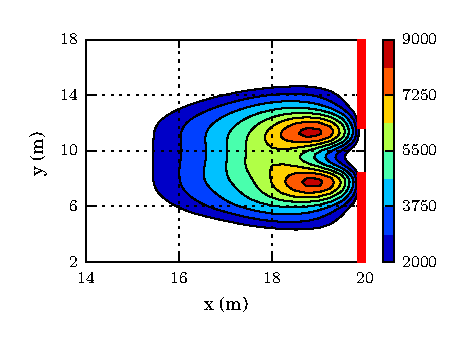
\includegraphics[width=0.75\columnwidth]{./fig4.eps}
% done with fig3_version0.py
}\hfill
\subfloat[Mean stream lines. The lines connect the normalized
velocity field ($v/v_\mathrm{max}$). The arrows indicate the stream 
direction.\label{fig:5}]{
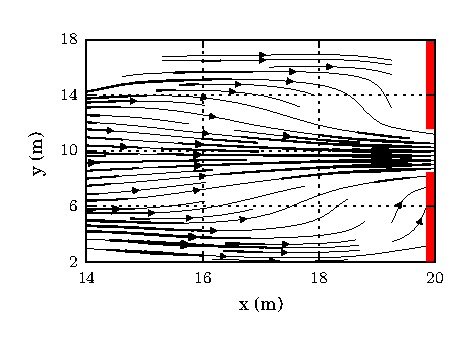
\includegraphics[width=0.75\columnwidth]{./fig5.eps}
% done with fig5_version0.py
}
\caption{\label{fig:3and5}Mean pressure and stream lines computed from 30 
evacuation processes until 100 pedestrians left the room 
($20\,\mathrm{m}\times20\,\mathrm{m}$ size). Data was recorded on a square grid 
of $1\,\mathrm{m}\times1\,\mathrm{m}$ and then splined to get smooth curves. 
The red lines at $x=20$~m represent the walls on the right of the room. 
There is only one opening of $3d_w=3.6$~m width (null separation distance 
between 
doors of width $3d_w/2$). The pedestrian's desired velocity was $v_d=4\,$m/s.}
\end{figure*}

%%%%%%%%%%% Flow figures %%%%%%%%%%%%%%%%%%%%%

\begin{center}
\CT
\subfloat[Opening of $d_w=1.2$~m width.]{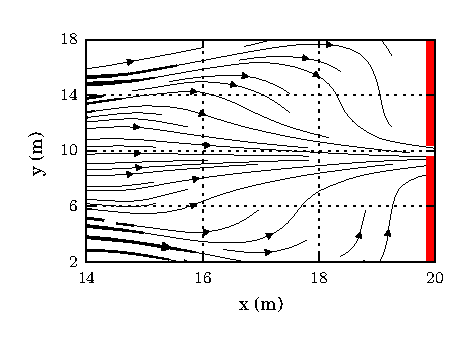
\includegraphics[width=0.75\columnwidth]{./flujo1_2_papercor.eps}}\quad
\subfloat[Opening of $2d_w=2.4$~m width.]{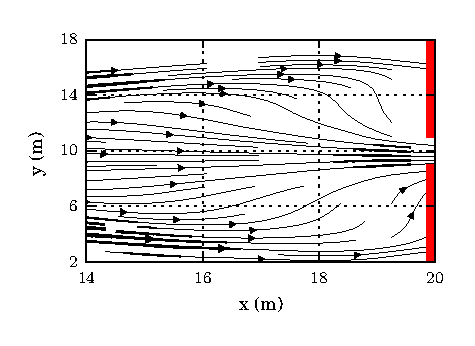
\includegraphics[width=0.75\columnwidth]{./flujo2_4_papercor.eps}}

\subfloat[Opening of $3d_w=3.6$~m width.]{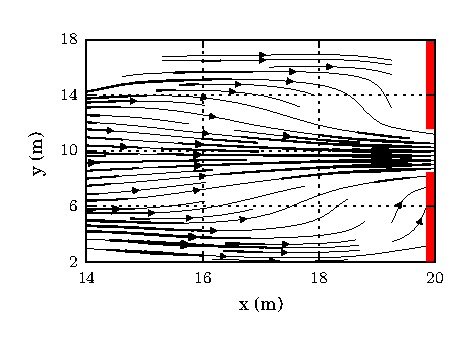
\includegraphics[width=0.75\columnwidth]{./fig5.eps}}\quad
\captionof{figure}{Mean stream lines computed from 30 
evacuation processes until 100 pedestrians left the room 
($20\,\mathrm{m}\times20\,\mathrm{m}$ size). The lines connect the normalized velocity field ($v/v_\mathrm{max}$). The arrows indicate the stream direction. Data was recorded on a square grid 
of $1\,\mathrm{m}\times1\,\mathrm{m}$ and then splined to get smooth curves. 
The red lines at $x=20$~m represent the walls on the right of the room. 
The pedestrian's desired velocity was $v_d=4\,$m/s for all the cases.}

\end{center}

%%%%%%%%%%%%%%%%%%%%%%%%%%%%%






We checked over the trajectory of the single pedestrian represented in 
Fig.~\ref{fig:8} and we observed that he (she) managed to get out of the room 
through the path where the stream lines get denser. Thus, Fig.~\ref{fig:8} 
resembles the stop-and-go process for the pedestrians passing through the 
middle of the clogging area, that is, along the low pressure (middle)
region. The pedestrians on the sides of this region (high pressure region) are 
expected to slow down since Fig.~\ref{fig:5} shows no stream lines to the exit. 
\\

Recalling the results in Fig.~\ref{fig:9} for the same single individual as in 
Fig.~\ref{fig:8}, we realize that the single door scene is likely 
to differ from the $d_g=0$ situation since both patterns (for the same 
individual) do. Thus, we examined the pressure contour map for the single door 
and for an opening of twice the single door width. The results are shown in 
Fig.~\ref{fig:2and4}. Fig.~\ref{fig:2} exhibits a similar pressure map pattern 
as Fig.~\ref{fig:3}, but the single door pressure map in Fig.~\ref{fig:4} does 
not. For the single door situation, we do not observe the lower pressure 
pathway in the middle of the clogging area. Instead, high pressure 
is acting on the pedestrians, as shown in the (normalized) pressure evolution 
in Fig.~\ref{fig:9}. The corresponding velocity evolution (Fig.~\ref{fig:9}) 
informs that the pedestrians in this region experience a slow down. \\

%%%%%%%%%%%%%%%% Pressure figures %%%%%%%%%%%%%%%%%%

\begin{center}
\CT
\subfloat[Opening of $d_w=1.2$~m width.\label{fig:4}]{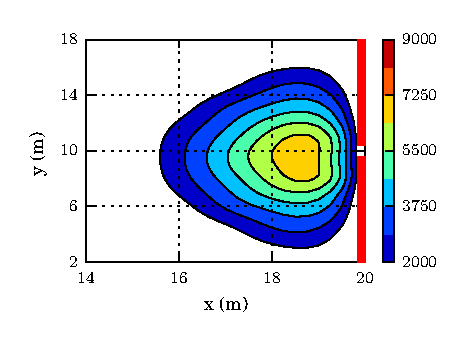
\includegraphics[width=0.75\columnwidth]{./fig6.eps}}\quad
\subfloat[Opening of $2d_w=2.4$~m width. \label{fig:2}]{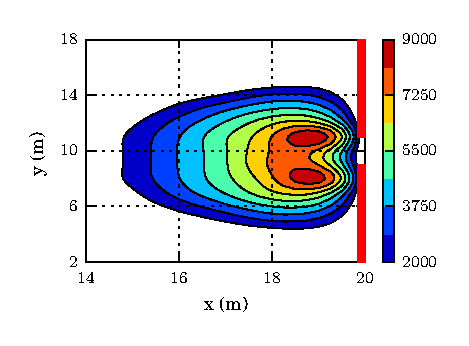
\includegraphics[width=0.75\columnwidth]{./fig7.eps}}

\subfloat[Opening of $3d_w=3.6$~m width. \label{fig:3}]{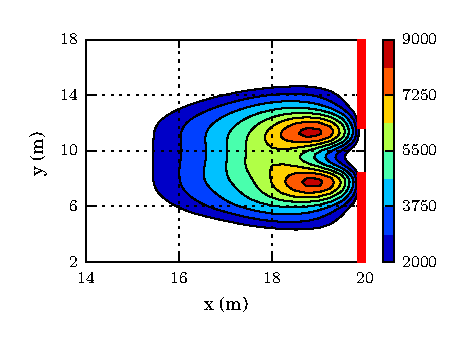
\includegraphics[width=0.75\columnwidth]{./fig4.eps}}\quad
\captionof{figure}{ Mean pressure contour lines computed from 30 evacuation processes until 100 pedestrians left the room ($20\,\mathrm{m}\times20\,\mathrm{m}$ size). The scale bar on the right is 
expressed in N.m$^{-1}$ units (see text for details). The red lines at $x=20$~m represent the walls on the right of the room. The pedestrian's desired velocity was $v_d=4\,$m/s. The contour lines were computed on a square grid of $1\,\mathrm{m}\times1\,\mathrm{m}$ and then splined to get smooth curves. Level colors can be seen in the on-line version only.}

\end{center}

%%%%%%%%%%%%%%%%%%%%%%%%%%%%%%%%%%

At this stage of the investigation we are able to point out a few conclusions. 
The widening of the single door increases the pedestrian's flux, as asserted in 
Ref.~\cite{daoliang1}. In the narrow situation (see Fig.~\ref{fig:9}), 
the pedestrians experience a slow down. The corresponding time delays have been 
associated to blocking structures (see Refs.~\cite{Dorso1,Dorso2}) and causes 
the pressure acting on the nearby individuals to rise. Fig.~\ref{fig:4} 
resembles this situation. However, as the opening widens (\emph{i.e.} the null 
separation situation), the pressure pattern changes qualitatively (see 
Fig.~\ref{fig:3} and Fig.~\ref{fig:2}), allowing the pedestrians in the middle 
of the clogging area to make a pathway to the exit. This pathway corresponds to 
the breaking of the blocking structures.   \\

\subsection{\label{door_seperation} Separated doors}

We will now analyze the case in which the evacuation process is through two 
doors, symmetrically placed on the same side of the room. We will explore the 
dependence of such a process on the doors separations. We will assume that 
each door width is $d_w=1.2\,$m.  \\

It has been shown in Fig.~\ref{fig:7} that separating the doors a distance 
$d_g=1\,$m worsens the evacuation performance with respect to the null 
separation. We  further explored this worsening by increasing $d_g$ at steps of 
$0.5\,$m, starting from the null separation distance. Fig.~\ref{fig:13} shows 
the mean evacuation time and the corresponding error bars (indicating the 
$\pm\sigma$ limits). The desired velocity was set to $v_d=4\,$m/s, where the 
``faster is slower'' effect takes place. \\

\begin{figure}
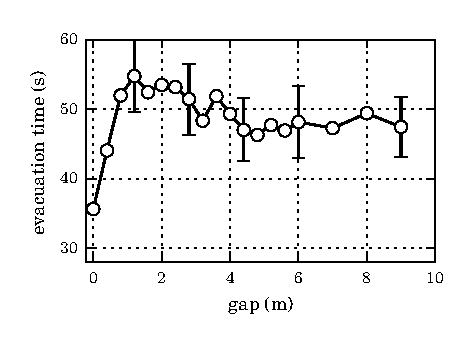
\includegraphics[width=\columnwidth]{./fig8.eps}
\caption{\label{fig:13} Mean evacuation time for 225 pedestrians (room of 
$20\times20$~m size) as a function of the doors separation distance. Mean 
values were computed from 30 evacuation processes until 160 pedestrians left 
the room. Each door was $d_w=1.2$~m width for non-vanishing gaps. The null gap 
means a single door of $2d_w$ width. The desired velocity was $v_d=4\,$m/s. }
% done with fig13_version0.py 
\end{figure}

The evacuation time as a function of $d_g$ shown in Fig.~\ref{fig:13} is one 
of our main results. The worsening in the evacuation performance rises to a 
maximum value at $1\,$m while its slope changes sign for $d_g>1\,$m. Thus, 
$d_g=1\,$m appears to be the worst evacuation scenario for the 
$20\,\mathrm{m}\times20\,\mathrm{m}$ room with 225 individuals and two 
doors of $d_w=1.2\,$m each (see Fig.~\ref{fig:13}).  \\


We further computed the mean evacuation time for an increasing number of 
pedestrians (and room sizes). We kept the pedestrian density unchanged (at 
$t=0$) for all the simulation processes. Fig.~\ref{fig:1} exhibits the mean 
evacuation time per pedestrian as a function of the separation distance 
(\emph{i.e.} gap). We divided the evacuation time by the total number of 
pedestrians for visualization reasons. \\


\begin{figure}
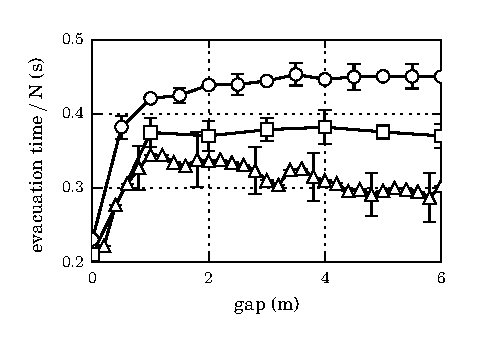
\includegraphics[width=\columnwidth]{./fig9.eps}
\caption{\label{fig:1} Mean evacuation time per total number of pedestrians 
that left the room ($N$), as a function of the doors separation distance. Mean 
values were computed from 30 evacuation processes. Each door was $d_w=1.2$~m 
width for non-vanishing gaps. The null gap means a single door of $2d_w$ width. 
Three situations are shown: $\bigtriangleup$ corresponds to the $20\times20$~m 
room when 160 pedestrians left the room, $\Box$ corresponds to $30\times30$~m 
room when 530 pedestrians left the room, and $\bigcirc$ corresponds to 
$40\times40$~m room when  865 pedestrians left the room. The desired velocity 
was $v_d=4\,$m/s. }
% done with fig1_version0.py 
\end{figure}

The results shown in Fig.~\ref{fig:1} were not expected. The evacuation time 
settles to an asymptotic value for separation distances $d_g>5\,$m. The mean 
evacuation time becomes almost independent of the separation distances $d_g$ 
despite that the clogging areas around the doors might still overlap. \\ 

Fig.~\ref{fig:1} also shows that the slope not always changes sign  
at $d_g\simeq1\,$m. Furthermore, as the number of pedestrians is increased for 
$d_g>1\,$m, the evacuation time slope raises to positive values. The 
greater the number of pedestrians, the worst the evacuation time (per 
individual). This appears to occur for $d_g>1\,$m, regardless of the crowd 
size. That is, according to Fig.~\ref{fig:1}, there exists a separation 
distance value $d_g\simeq1\,$m where the evacuation slope changes sharply 
to negative or positive values (for $d_g>1\,$m). This phenomenon has not been 
studied in the literature, to our knowledge. \\

We can resume the results in Fig.~\ref{fig:1} in the following way: the 
evacuation time rises when the doors separation increases from a wide opening 
(null separation distance) to the distance $d_g\simeq1\,$m. At this gap, the 
evacuation time slope changes notably, entering a much slowly 
varying regime towards an asymptotic value (for $d_g\gg1\,$m).  The former can 
be identified as a regime for small values of $d_g$, while the latter is valid 
for moderate to large values of $d_g$. The fact that a sharp change occurs at 
$d_g\simeq1\,$m, no matter the crowd size, suggests that both regimes are 
somehow different in nature. This moved us to explore the two regimes 
separately. \\

\subsubsection{\label{small_regime} The regime for $d_g<1\,$m}

Our starting point is the pressure contour map, since we can easily compare the 
current patterns with those presented in Section~\ref{null_gap_patterns}. 
Fig.~\ref{fig:16} shows the mean pressure pattern for the separation distance 
$d_g=1.5\,$m, that is, close to the gap value where the sharp change in the 
slope occurs. The differences between Fig.~\ref{fig:16} and 
Fig.~\ref{fig:2and4} are noticeable. We can now see a wide region in the center of 
the clogging area representing the high pressure ($P_i$) acting 
on each pedestrian (warm colors in Fig.~\ref{fig:16}). The regularity in the 
colors of this region is meaningful: the high pressure acting on the pedestrians 
does not allow a regular stream (pathway) to the exit. This is in agreement with 
the evacuation time worsening shown in Fig.~\ref{fig:13}.   \\

% {\color{red} In all cases the pressure maps showed a resemblance with the ones reported
%in~\cite{Zhang}}

\begin{figure*}[!htbp]
\subfloat[Separation distance of $d_g=1.5$~m.\label{fig:16}]{
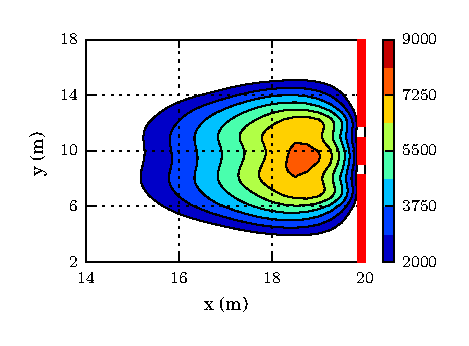
\includegraphics[width=0.75\columnwidth]{./fig10.eps}
% done with fig16_version0.py 
}\hfill
\subfloat[Separation distance of $d_g=5$~m. \label{fig:17}]{
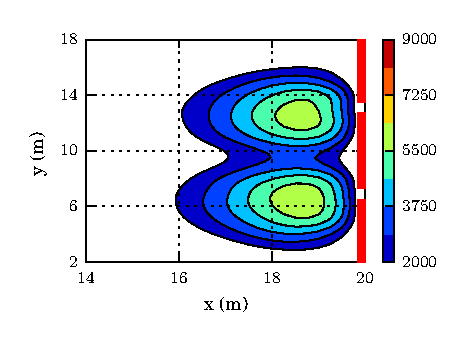
\includegraphics[width=0.75\columnwidth]{./fig11.eps}
% done with fig17_version0.py 
}
\caption{\label{fig:16and17} Mean pressure contour lines computed from 30 
evacuation processes until 100 pedestrians left the room 
($20\,\mathrm{m}\times20\,\mathrm{m}$ size). The scale bar on the right is 
expressed in N.m$^{-1}$ units (see text for details). The red lines at 
$x=20$~m represent the walls on the right of the room. The pedestrian's desired 
velocity was $v_d=4\,$m/s. The contour lines were computed on a square grid of 
$1\,\mathrm{m}\times1\,\mathrm{m}$ and then splined to get smooth curves. Level 
colors can be seen in the on-line version only.} 
\end{figure*}


Fig.~\ref{fig:16} suggests that blocking structures might be present for long 
time periods, since the pedestrians cannot manage to get out easily. We 
examined this possibility through the \textit{blocking probability}. In this 
context, the blocking probability is associated to the ratio between the time 
that each door remains blocked with respect to the total evacuation time (cf. 
Section~\ref{human}). Fig.~\ref{fig:14} presents two kinds of blockings: the 
simultaneous blocking of both doors, and the blocking of a single door (say, 
the one on the left). The former connects the left most wall with the right 
most wall, but does not contact the separation wall in the middle of the walls. 
The latter connects the walls on both sides of the selected door (say, 
the one on the left). \\


\begin{figure}
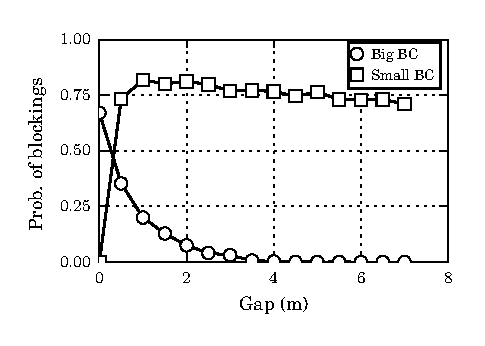
\includegraphics[width=\columnwidth]{./fig12.eps}
\caption{\label{fig:14} Ratio between time steps including blocking structures 
and the total number of time steps for 30 evacuation processes, as a function 
of the doors separation distance. The room size was $20\times20$~m with 225 
occupants. Each door was $d_w=1.2$~m width for non-vanishing gaps. The null gap 
means a single door of $2d_w$ width. The desired velocity was $v_d=4\,$m/s.  
$\bigcirc$ corresponds blocking structures connecting both the left side wall 
of the left door with the right side wall of the right door (see text for 
details). $\Box$ corresponds to blocking structures connecting both sides of a 
single door (see text for details).   }
% done with fig14_version0.py 
\end{figure}

According to Fig.~\ref{fig:14}, the single door blockings are not relevant 
until $d_g\simeq1\,$m, while the simultaneous blockings weaken as the gap 
(separation distance $d_g$) increases. The single door blockings resemble the 
response in Fig.~\ref{fig:13}, and thus, we conclude that this kind of 
blockings should play an important role in the increase of the evacuation time 
for small gaps $d_g$. Notice that single door blocking probability explains the 
75\% of the evacuation time, as can be seen in Fig.~\ref{fig:14}. \\

The results so far moved us to focus closer on the dynamics around each door. 
We watched many animations of the evacuation process for gap distances between 
the null separation to $d_g=1.5\,$m (not shown). We realized that single 
door blockings hold if the gap is large enough to accommodate at least two 
pedestrians. That is, any blocking structure enclosing a single door can hold 
for some time if the pedestrians at the end of the structure (and in contact 
with the walls) do hardly leave the structure. Two pedestrians are needed at the 
gap wall to ensure that both doors remain blocked.\\ 

We want to call the attention on the fact that when $d_g$ passes through the 
$1\,$m situation, the kind of simultaneous blocking without contacting the gap 
wall, is replaced by the kind of single door blockings acting (usually) 
simultaneously. This achieves a qualitative different pressure and 
stream pattern. As shown in Fig.~\ref{fig:2}, the widening of the exit 
allows a pathway through the middle of the clogging area. This is likely to 
occur even for very small gaps (see Fig.~\ref{fig:14}). However, the single door 
blockings follow a pressure pattern similar to  Fig.~\ref{fig:4} on each door.  
What we see in Fig.~\ref{fig:16} is the combined pattern built from two 
single door patterns as in Fig.~\ref{fig:4}. \\

We conclude from the analysis of small gaps ($d_g<1\,$m) that a door 
separation distance roughly equal to two pedestrian widths is critical. 
This distance allows persistent single door blockings. Small distances (close 
to the null separation) do not actually allow single door blockings to hold for 
long time. Thus, the role of $d_g=2r_{ij}$ (two pedestrian's width) is decisive to move the evacuation 
process from one regime to another. \\ 


\subsubsection{\label{large_regime} The regime for $d_g>1\,$m}

Fig.~\ref{fig:14} shows that the single door blockings (see 
 Section~\ref{small_regime}) remains around 75\% of the total evacuation time 
for $d_g>1\,$m (225 individuals in the room). We also computed this magnitude 
for situations with increasing number of individuals (see Fig.~\ref{fig:15}). 
The probability of single door blockings approaches unity as the crowd size 
increases. This means, according to our definition of blocking probability, 
that the blocking time raises as the number of individuals increases. The gap 
distance, however, does not play a significant role for $d_g>1\,$m.  \\ 


\begin{figure}
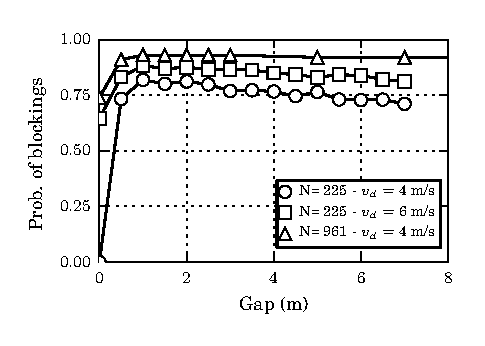
\includegraphics[width=\columnwidth]{./fig13.eps}
\caption{\label{fig:15} Ratio between time steps including blocking structures 
and the total number of time steps for 30 evacuation processes, as a function 
of the doors separation distance. The only blocking structures considered 
were those connecting both sides of one single door (see text for details). 
Each door was $d_w=1.2$~m width for non-vanishing gaps. The null gap means a 
single door of $2d_w$ width. Three scenarios are shown: $\bigcirc$ 
corresponds to the room of size $20\times20$~m with 225 occupants and a 
desired velocity of $v_d=4\,$m/s. $\Box$ corresponds to the room of size  
$20\times20$~m with 225 occupants and a desired velocity of $v_d=6\,$m/s. 
$\bigtriangleup$ corresponds to the room of size $40\times40$~m with 961 
occupants and a desired velocity of $v_d=4\,$m/s.   }
% done with fig15_version0.py 
\end{figure}

There is a noticeable difference between the evacuation time 
shown in Fig.~\ref{fig:1} and the blocking probability exhibited in 
Fig.~\ref{fig:15}. Fig.~\ref{fig:1} presents the evacuation time for three 
different room sizes and increasing number of pedestrians.  The slope of the 
evacuation curve is negative for the $20\times20\,$m room, it vanishes for 
the $30\times30\,$m situation and it becomes slightly positive for the 
$40\times40\,$m room (for $d_g>1\,$m). Thus, as the number of pedestrians 
increases, the slope of the evacuation time changes sign. However, this does not 
occur for the blocking probability (see Fig.~\ref{fig:15}). The slope of the 
blocking probability remains always negative for an increasing number of 
pedestrians (and desire velocities). Therefore, the changes in the slope 
observed in Fig.~\ref{fig:1} cannot be explained by changes in the blocking 
time (\textit{i.e} blocking probability).   \\

We checked the pressure patterns for $d_g>4d_w$ (see Fig.~\ref{fig:17} as an 
example). We came to the conclusion that since the evacuation slope in 
Fig.~\ref{fig:1} changes with an increasing number of individuals, the whole 
bulk should be involved in this phenomenon. Therefore, we focused our 
investigation on the pressure contribution of the whole bulk.  \\ 

As shown in Eq.~(\ref{eqn_5}) of \ref{alternative} , we can realize that the pressure of the 
whole bulk (left-hand side) is related to the total desire force contribution 
(right-hand side). Thus, the pressure of the bulk can vary in two possible 
ways: if the desire force of the individuals (\emph{i.e.} anxiety levels) 
changes, or, if the crowd size changes. An increase on either 
the number of evacuating pedestrians ($N$) or their corresponding anxiety 
level ($v_d$), will increase the pressure of the whole bulk % {\color{red} this result
% is in accordance with the experiment performed by Jose M. Pastor et al. in~\cite{Pastor}.}
A simple example is presented in the Appendix. \\

Fig.~\ref{fig:1} exhibits the evacuation time for an increasing number of 
pedestrians. But, an increase in the pedestrians anxiety level should  
resemble similar results, if the above reasonings are true. Fig.~\ref{fig:12} 
shows the evacuation time as a function of the separation distance for two 
different desired velocities. As expected, the sharp change in the slope occurs 
around $d_g=2r_{ij}$. Also the slope changes as the desired velocity ($v_d$) is 
increased (\emph{i.e.} higher anxiety level). This confirms that the social 
pressure is responsible the slope behaviour shown in Fig.~\ref{fig:1}. \\


\begin{figure}
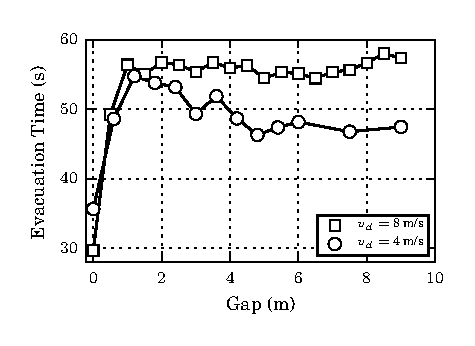
\includegraphics[width=\columnwidth]{./fig14.eps}
\caption{\label{fig:12} Mean evacuation time for 225 pedestrians (room of 
$20\times20$~m size) as a function of the doors separation distance. Mean 
values were computed from 30 evacuation processes until 160 pedestrians left 
the room. Each door was $d_w=1.2$~m width for non-vanishing gaps. The null gap 
means a single door of $2d_w$ width. $\bigcirc$ corresponds to pedestrians 
with desired velocity of $v_d=4\,$m/s. $\Box$ corresponds to pedestrians 
with desired velocity of $v_d=8\,$m/s. }
% done with fig12_version0.py 
\end{figure}


We conclude from the analysis of large gaps ($d_g>1\,$m) that the evacuation 
time is controlled by the social pressure in the bulk. The crowd size and 
the desired velocity $v_d$ affects the pressure acting on the pedestrians. 
For $d_g>5\,$m in our simulations, the evacuation time is very close to the 
corresponding asymptotic value, although the bulks around each door are not 
completely independent. This means that the mixing of both crowds (that is, 
the fact that the bulks are in contact) do not affect strongly the evacuation 
performance.   \\





